\begin{figure}[!htb]
\begin{center}
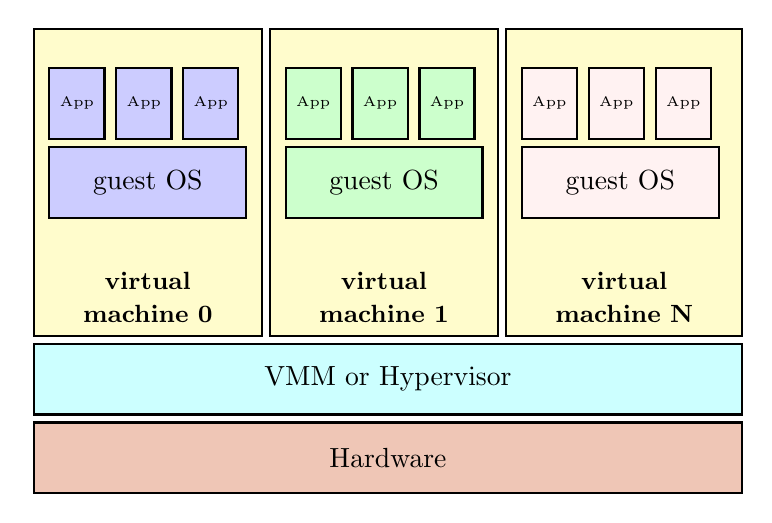
\begin{tikzpicture}

\node at (0,2) [rectangle, draw=black, thick, fill=yellow!20, minimum height = 3.9cm, minimum width = 2.9cm, anchor=south west] (vm0) {};
\node [above, inner sep=5pt, align=center, text width=2.7cm] at (vm0.south) {\textbf{\small{virtual\\ machine 0}}};

\node at (0.2,3.5) [rectangle, draw=black, thick, fill=blue!20, minimum height = 0.9cm, minimum width = 2.5cm, anchor=south west] (g0) {guest OS};
\node at (0.2,4.5) [rectangle, draw=black, thick, fill=blue!20, minimum height = 0.9cm, minimum width = 0.7cm, anchor=south west] (g0app0) {\tiny{App}};
\node at (0.2+0.85,4.5) [rectangle, draw=black, thick, fill=blue!20, minimum height = 0.9cm, minimum width = 0.7cm, anchor=south west] (g0app1) {\tiny{App}};
\node at (0.2+1.7,4.5) [rectangle, draw=black, thick, fill=blue!20, minimum height = 0.9cm, minimum width = 0.7cm, anchor=south west] (g0appn) {\tiny{App}};

\node at (3,2) [rectangle, draw=black, thick, fill=yellow!20, minimum height = 3.9cm, minimum width = 2.9cm, anchor=south west] (vm1) {};
\node [above, inner sep=5pt, align=center, text width=2.7cm] at (vm1.south) {\textbf{\small{virtual\\ machine 1}}};
\node at (3.2,3.5) [rectangle, draw=black, thick, fill=green!20, minimum height = 0.9cm, minimum width = 2.5cm, anchor=south west] (g1) {guest OS};
\node at (3.2,4.5) [rectangle, draw=black, thick, fill=green!20, minimum height = 0.9cm, minimum width = 0.7cm, anchor=south west] (g1app0) {\tiny{App}};
\node at (3.2+0.85,4.5) [rectangle, draw=black, thick, fill=green!20, minimum height = 0.9cm, minimum width = 0.7cm, anchor=south west] (g1app1) {\tiny{App}};
\node at (3.2+1.7,4.5) [rectangle, draw=black, thick, fill=green!20, minimum height = 0.9cm, minimum width = 0.7cm, anchor=south west] (g1appn) {\tiny{App}};

\node at (6,2) [rectangle, draw=black, thick, fill=yellow!20, minimum height = 3.9cm, minimum width = 3cm, anchor=south west] (vmn) {};
\node [above, inner sep=5pt, align=center, text width=2.7cm] at (vmn.south) {\textbf{\small{virtual\\ machine N}}};
\node at (6.2,3.5) [rectangle, draw=black, thick, fill=pink!20, minimum height = 0.9cm, minimum width = 2.5cm, anchor=south west] (gn) {guest OS};
\node at (6.2,4.5) [rectangle, draw=black, thick, fill=pink!20, minimum height = 0.9cm, minimum width = 0.7cm, anchor=south west] (gnapp0) {\tiny{App}};
\node at (6.2+0.85,4.5) [rectangle, draw=black, thick, fill=pink!20, minimum height = 0.9cm, minimum width = 0.7cm, anchor=south west] (gnapp1) {\tiny{App}};
\node at (6.2+1.7,4.5) [rectangle, draw=black, thick, fill=pink!20, minimum height = 0.9cm, minimum width = 0.7cm, anchor=south west] (gnappn) {\tiny{App}};

\node at (0,1) [rectangle, draw=black, thick, fill=Cyan!20, minimum height = 0.9cm, minimum width = 9cm, anchor=south west] (hyper) {VMM or Hypervisor};
\node at (0,0) [rectangle, draw=black, thick, fill=BrickRed!20, minimum height = 0.9cm, minimum width = 9cm, anchor=south west] (hard) {Hardware};


\end{tikzpicture}
\end{center}
\ifreport
\caption{Virtualization Technology}
\fi
\label{fig-virtualization}
\end{figure}
